\documentclass[11pt]{article}

\usepackage{a4wide}
\usepackage[utf8]{inputenc}
\usepackage[T2A]{fontenc}
\usepackage[russian]{babel}
\usepackage{graphicx}
\usepackage{color}
\usepackage[left=2.5cm,right=2.5cm,
    top=2.5cm,bottom=2.5cm,bindingoffset=0cm]{geometry}
\usepackage {amsthm}
\usepackage {amsmath}
\usepackage{amssymb}

\newtheorem{Def}{Определение}
\newtheorem{statement}{Утверждение}
\newtheorem{theorem}{Теорема}
\newenvironment{Proof}
{\par\noindent{\bf Доказательство.\\}} 
{\begin{flushright}$\Box$\end{flushright}}

\definecolor{gray}{rgb}{0.5,0.5,0.5}

\newcommand\Set[2]{\left\{ #1 \mid #2 \right\}}
\newcommand\Ref[1]{(\ref{#1})}
\newcommand\ftw[2]{\overline{#1,#2}}
\newcommand\RS{\Ref{system} }
\newcommand\beq{\begin{equation}}
\newcommand\eeq{\end{equation}}
\newcommand\dd[2]{\frac{\partial#1}{\partial#2}}


\begin{document}

\thispagestyle{empty}

\begin{center}
\ \vspace{-3cm}

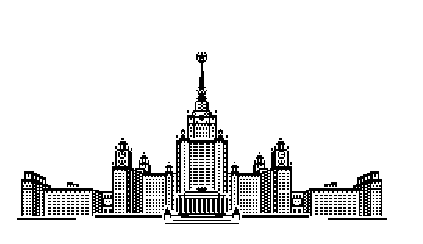
\includegraphics[width=0.5\textwidth]{msu.eps}\\
{\scshape Московский государственный университет имени М.~В.~Ломоносова}\\
Факультет вычислительной математики и кибернетики\\
Кафедра системного анализа

\vfill

{\LARGE Выпускная квалификационная работа по теме}

\vspace{1cm}

{\Huge\bfseries <<Управление в моделях межвидового взаимодействия>>}
\end{center}

\vspace{1cm}

\begin{flushright}
  \large
  \textit{Студентка 415 группы}\\
  Т.~Е.~Морозова
  \textit{Научный руководитель}\\
  к.ф.-м.н., доцент И.~В.~Рублёв 

  \vspace{5mm}

 \end{flushright}

\vfill

\begin{center}
Москва, 2018
\end{center}

\newpage
\tableofcontents
\newpage

%=============Введение============
\section{Введение}

Рассматривается модель пищевой цепи с управлением без внутривидовой конкуренции, состоящая из четырех звеньев и описываемая следующей системой:

\beq
\left\{
\begin{aligned}
\label{system}
	\dot x_1 &= x_1(r_1 + u_1- b_1x_2), \\
	\dot x_2 &= x_2(-r_2 - b_2x_3 + c_2x_1), \\
	\dot x_3 &= x_3(-r_3 + u_2 - b_3x_4 + c_3x_2), \\
	\dot x_4 &= x_4(-r_4 + c_4x_3).
\end{aligned}
\right.
\eeq

Здесь $x_i,\, i = \ftw{1}{4}$ --- численности популяций видов, $r_1 + u_1$ --- рождаемость первого вида,  $r_2, r_3-u_2, r_4$ --- смертности остальных видов, $b_1, b_2, b_3$ и $c_2, c_3, c_4$ отвечают за взаимодействие между популяциями. Все параметры строго положительны, а управления берутся из интервалов $U_1^* = [u_1^{min}, u_1^{max}], U_2^* = [u_2^{min}, u_2^{max}]$ соответственно.

В данной работе основной целью является исследование свойств и синтеза управления для задачи быстродействия во множество положений равновесия.

%=============Общие свойства===========
\section{Общие свойства системы}

Из биологической интерпретации вытекает, что численность популяции не может быть отрицательной. В следующем утверждении будет показано, что система удовлетворяет этому свойству.

\begin{statement}
	Множество $\Set{x \in \mathbb{R}^4}{x_i > 0, i = \ftw{1}{4}}$ инвариантно относительно системы \RS.
\end{statement}
\begin{Proof}
	Из системы \RS видно, что при обнулении координат, обнуляются соответственно и выражения для $\dot x_i,$ так что координаты не могут поменять знак. Интегрируя в обратном времени, получим, что координаты не могут обнулиться.
\end{Proof}

Рассмотрим положения равновесия \RS как функцию управления: 
\begin{gather}
	P(u) = (P_1(u), P_2(u), P_3(u), P_4(u)),\; \text{где} \notag \\
	P_1(u) = \frac{r_2c_4 + b_2r_4}{c_2c_4}, \;\; P_2(u) = \frac{r_1 + u_1}{b_1}, \;\; P_3(u) = \frac{r_4}{c_4},\;\; P_4(u) = \frac{c_3(r_1+u_1) + (u_2 - r_3)b_1}{b_1b_3}.
\end{gather}

Заметим, что от управления существенно зависят только вторая и четвертая координата, поэтому в дальнейшем будем обозначать $P(u) = (P_1, P_2(u), P_3, P_4(u)).$ \\

Множество положений равновесия $E = \Set{P(u)}{u \in U^*}$ представляет из себя параллелограмм в пространстве $(x_2, x_4).$ В нашей работе мы предполагаем его непустоту, для этого введем ограничение на параметры задачи:
$$P_4(u_1^{min}, u_2^{min}) > 0.$$

Наша задача состоит в исследовании возможности перевода системы \RS во множество $E$ при кусочно-непрерывном управлении из $U_1^*, U_2^*.$ 

В работе \cite{MathBio} найден первый интеграл системы \RS:
\beq
	K(x,u) = x_1 - P_1\ln x_1 + \frac{b_1}{c_2}(x_2 - P_2(u)\ln x_2) + \frac{b_1b_2}{c_2c_3}(x_3 - P_3\ln x_3) + \frac{b_1b_2b_3}{c_2c_3c_4}(x_4 - P_4(u)\ln x_4).
\eeq

Докажем, что функция $K(x,u)$ сильно выпукла по $x$ и имеет минимум по $x$ в точке $(P(u),u).$

\begin{statement}
	Функция $K(x,u)$ сильно выпукла на любом выпуклом ограниченном подмножестве $\mathbb{R}_+^4,$ а ее глобальный минимум по $x$ достигается в точке $(P(u),u).$
\end{statement}
\begin{Proof}
	Рассмотрим гессиан функции $K(x,u):$
	$$H = \text{diag} \left(\frac{P_1}{x_1^2}, \; \frac{P_2(u)b_1}{c_2x_2^2}, \; \frac{P_3b_1b_2}{c_2c_3x_3^2}, \; \frac{P_4(u)}{c_2c_3c_4x_4^2}\right).$$
	Очевидно, он больше нуля при всех $x_i > 0,$ следовательно, функция выпукла.\\
	Обозначим 
	$$K_1(x_1) = x_1 - P_1\ln x_1, \; K_2(x_2,u) = \frac{b_1}{c_2}(x_2 - P_2(u)\ln x_2),$$
	$$K_3(x_3) = \frac{b_1b_2}{c_2c_3}(x_3 - P_3\ln x_3), \; K_4(x_4,u) = \frac{b_1b_2b_3}{c_2c_3c_4}(x_4 - P_4(u)\ln x_4,$$ тогда $K(x,u) =  K_1(x_1) + K_2(x_2,u) + K_3(x_3) + K_4(x_4,u).$  Поскольку 
	$$K_1'(x_1) = 1 - \frac{P_1}{x_1}, \; K_2'(x_2,u) = \frac{b_1}{c_2} - \frac{P_2(u)b_1}{c_2x_2},$$
	$$K_3'(x_3) = \frac{b_1b_2}{c_2c_3} - \frac{b_1b_2P_3}{c_2c_3x_3}, \; K_4(x_4,u) = \frac{b_1b_2b_3}{c_2c_3c_4} - \frac{b_1b_2b_3P_4(u)}{c_2c_3c_4x_4},$$ 
	глобальный минимум $K_i$ достигается при $x_i = P_i,$ следовательно, глобальный минимум $K(x,u)$ достигается в точке $(P(u),u).$ \\
	 Докажем сильную выпуклость. Возьмем $x_i \leqslant \mu, i = \ftw{1}{4}, \text{где } \mu \geqslant \max\Set{P_i}{i = \ftw{1}{4}}.$ Тогда $H \geqslant \delta\cdot I,$ где  
	 $$\delta = \min\left(P_1, \frac{P_2(u)b_1}{c_2}, \frac{P_3b_1b_2}{c_2c_3}, \frac{P_4(u)b_1b_2b_3}{c_2c_3c_4}\right)/\mu^2.$$
	 Таким образом $\langle Hx,x \rangle \geqslant \langle \delta Ix,x \rangle = \delta \|x\|^2,$ что и завершает доказательство.
\end{Proof}



%Введем функцию $\tilde K(x,u) = K(x,u) - K(P(u),u).$ Очевидно, она также сильно выпукла, неотрицательна и равна нулю в точке минимума $(P(u),u).$ Таким образом, наша задача сводится к поиску минимума функции $\tilde K(x,u)$ по $u$ из $U^*.$\\
%\textcolor{blue}{Вообще пока нет особого смысла в $\tilde K(x,u).$ Или есть?.. Тут надо доказать как-то, что если $u^*(t) \in \bar U^* : K(x,u^*) \leqslant K(x,u)\; \forall x, \forall u \in U^*, \text {то } \exists t > t_0 : x(t,t_0,x_0 \mid u*) \in E, \;\; \bar U^* = \Set{u(t)}{u(t) \in U^* \forall t}.$}
%
%Таким образом, будем искать $\min\limits_{u(t) \in \bar U^*} K(x,u).$ 
%Посчитаем производную:
%$$\frac{dK(x,u)}{du} = -(P_2)'_u\frac{b_1}{c_2}\ln x_2 - (P_4)'_u\frac{b_1b_2b_3}{c_2c_3c_4}\ln x_4 = -\frac{c_4\ln x_2 + b_2\ln x_4}{c_2c_4}.$$
%Видим, что минимум достигается на кривой 
%\beq
%	x_2 = x_4^{-\frac{b_2}{c_4}}.
%\eeq
%\textcolor{blue}{Видимо, это кривая переключения управления???.\\}
%
%Проверим, есть ли на этой кривой неподвижные точки:
%$$
%	\left\{
%	\begin{aligned}
%		x_4 &= x_2^{-\frac{c_4}{b_2}}, \\
%		x_4 &= \frac{c_3x_2 - r_3}{b_3}
%	\end{aligned}
%	\right.
%$$
%Так как все параметры задачи положительны, то эти кривые имеют ровно одну точку пересечения в области $x_2 > 0, x_4 > 0.$

%Будем искать $\min\limits_{u \in U^*} K(x,u).$ 
%он каким-то хуем приведет нас в положение равновесия. 

%Особые режимы
\begin{statement}
	В системе (1) в области $\mathbb{R}_+^4$ не могут возникать особые режимы управления.
\end{statement}
\begin{Proof}
    Выпишем функцию Гамильтона-Понтрягина для нашей системы.
        $$H(\psi, x, u) = \psi_1x_1(r_1 + u_1 - b_1x_2) + \psi_2x_2(-r_2 - b_2x_3 + c_2x_1) + \psi_3x_3(-r_3 + u_2 - b_3x_4 + c_3x_2) + \psi_4x_4(-r_4 + c_4x_3),$$
    
    где  $\psi(t) \in C, \; \psi(t) \ne 0 \; \text{и удовлетворяет сопряженной системе системе:}$
    
    $$
    \left\{
    \begin{aligned}
    	\dot \psi_1 &= -(\psi_1(r_1 + u - b_2x_2) + \psi_2x_2c_2), \\
    	\dot \psi_2 &= -(-b_1\psi_1x_1 + \psi_2(-r_2 - b_2x_3 + c_2x_1) + \psi_3x_3c_3), \\
    	\dot \psi_3 &= -(-b_2\psi_2x_2 + \psi_3(-r_3 + u_2 - b_3x_4 + c_3x_2) + \psi_4x_4c_4), \\
    	\dot \psi_4 &= -(b_3\psi_3x_3 + \psi_4(-r_4 + c_4x_3)).
    \end{aligned}
    \right.$$
    
    Из принципа максимума $H(\psi(t), x(t), u^*(t)) = \sup\limits_{u \in U^*} H(\psi,x,u).$
    
    Посчитаем производную $H$ по $u:$
    
    $$H'_u = (\psi_1x_1, \psi_3x_3) \text{ откуда } u_1^* = \begin{cases} u_1^{max}, & \psi_1x_1 \geqslant 0, \\  u_1^{min}, & \psi_1x_1 < 0.\end{cases}, \;\; u_2^* = \begin{cases} u_2^{max}, & \psi_3x_3 \geqslant 0, \\  u_2^{min}, & \psi_3x_3 < 0.\end{cases}$$
    
    Особый режим будет возникать, если хотя бы одна из компонент управления определяется неоднозначно, то есть либо $\psi_1x_1 = 0,$ либо $\psi_3x_3 = 0$ на ненулевом промежутке времени.
    Так как в нашей системе $x_1$ и $x_3$ положительны, учитываются только $\psi_1, \psi_3.$  
    
    Рассмотрим оба варианта.
    \begin{enumerate}
    \item
        	Пусть $\psi_1(t) = 0, t \in [t_1 t_2].$ Рассмотрим последовательно $\dot \psi_i$ и убедимся, что все сопряженные переменные нулевые.
        
        Если $\psi_1(t) = 0$ на промежутке $[t_1, t_2],$ то $\dot \psi_1 = 0$ на этом же временном отрезке. Но тогда из первого сопряженного уравнения $\psi_2 = 0,$ следовательно и $\dot \psi_2 = 0, \;  t \in [t_1, t_2],$ а тогда из второго сопряженного уравнения $\psi_3 = 0, \;  t \in [t_1, t_2].$ Аналогично $\dot \psi_3 = 0, \;  t \in [t_1, t_2]$ и из третьего сопряженного уравнения $\psi_4 = 0, \;  t \in [t_1, t_2],$ что противоречит невырожденности $\psi(t).$
        
    \item
    	Пусть $\psi_3(t) = 0, \psi_1(t) \ne 0, t \in [t_1 t_2],$ тогда и $\dot \psi_3(t) = 0$ на том же временном отрезке. Таким образом $-b_2\psi_2x_2 + \psi_4x_4c_4 = 0.$ Возьмем производную по времени от этого выражения:
    	\begin{multline*}
    		0 = -b_2(\dot \psi_2x_2 + \psi_2 \dot x_2) + c_4(\dot \psi_4 x_4 + \psi_4 \dot x_4) = \\
    		= -b_2(-x_2(-b_1\psi_1x_1 + \psi_2(-r_2 - b_2x_3 + c_2x_1)) + \psi_2 x_2(-r_2 - b_2x_3 + c_2x_1)) + \\
    		+ c_4(\psi_4x_4(-r_4 + c_4x_3) + \psi_4x_4(-r_4 + c_4x_3)) = -b_1b_2x_1x_2\psi_1.
    	\end{multline*}
    	
    	Но $x_1, x_2, \psi_1 \ne 0,$ а значит, мы получили противоречие, что и завершает доказательство.
    
    \end{enumerate}    
\end{Proof}

%Вернемся к нашим баранам
Вернемся к $K(x,u).$ Уменьшая ее, мы будем приближаться к положению равновесия. 
Посчитаем производную $\frac{dK(x,u^0)}{dt}$ при некотором $u^0 = (u_1^0, u_2^0)$ в силу системы \RS:

\begin{multline*}
    \frac{dK(x,u_0)}{dt} = \dd{K(x,u_0)}{x_1}\dot x_1 + \dd{K(x,u_0)}{x_2}\dot x_2 + \dd{K(x,u_0)}{x_3}\dot x_3 + \dd{K(x,u_0)}{x_4}\dot x_4 = \\
    = -\frac{1}{c_2c_3c_4}\left((u_2 - u_2^0)(b_1b_2(r_4 - c_4x_3)) + c_3(u_1 - u_1^0)(b_2r_4 + c_4r_2 - c_2c_4x_1)\right) = \\
    = \frac{b_1b_2}{c_2c_3}(u_2 - u_2^0)(x_3 - P_3) + (u_1 - u_1^0)(x_1 - P_1).
\end{multline*}

Заметим, что равновесие по $x_1$ и $x_3$ разделяет все пространство на четыре области, в каждой из которых будет свой минимизатор.
\begin{enumerate}
\item
	В области $x_1 > P_1, \, x_3 > P_3$ производная будет минимальной при $u_1 = u_1^{min}, \, u_1^0 = u_1^{max}, \, u_3 = u_3^{min}, \, u_3^0 = u_3^{max}.$
\item
	В области $x_1 > P_1, \, x_3 < P_3$ производная будет минимальной при $u_1 = u_1^{min}, \, u_1^0 = u_1^{max}, \, u_3 = u_3^{max}, \, u_3^0 = u_3^{min}.$
\item
	В области $x_1 < P_1, \, x_3 > P_3$ производная будет минимальной при $u_1 = u_1^{max}, \, u_1^0 = u_1^{min}, \, u_3 = u_3^{min}, \, u_3^0 = u_3^{max}.$
\item
	В области $x_1 < P_1, \, x_3 < P_3$ производная будет минимальной при $u_1 = u_1^{max}, \, u_1^0 = u_1^{min}, \, u_3 = u_3^{max}, \, u_3^0 = u_3^{min}.$
\end{enumerate}

Введем 4 функции:
$$K_1(x) = K(x,u_1^{min}, u_2^{min}), \, K_2(x) = K(x,u_1^{max}, u_2^{min}),$$ 
$$K_3(x) = K(x,u_1^{min}, u_2^{max}), \, K_4(x) = K(x,u_1^{max}, u_2^{max}).$$

Беря управление, минимизирующее производную $\frac{dK, u^0}{dt}$ в соответствующей области, мы будем уменьшать три функции, а четвертая будет постоянной. Процесс будет повторяться до тех пор, пока мы не попадем на положение равновесия, где все четыре функции станут постоянными.

%=========Скользящие режимы========

Однако неопределенность возникает на самих гиперповерхностях $x_1 = P_1, x_3 = P_3.$ Если возникает скользящий режим, то управлять системой становится затруднительно ввиду неоднозначности управления. 

Рассмотрим подробнее, когда возникают скользящие режимы. Перепишем нашу систему в виде:
$$\dot x(t) = \begin{cases} f_1(x), & \sigma(x,t) < 0 \\ f_2(x), & \sigma(x,t) > 0.\end{cases}$$
Достаточное условие скользящего режима на отрезке $x \in [a, b]$ в этом случае будет:
$$
\left\{
\begin{aligned}
    \lim_{\sigma \to 0+0}\dd{\sigma(x,t)}{x} f_2(x) < 0 \\
    \lim_{\sigma \to 0-0} \dd{\sigma(x,t)}{x} f_1(x) > 0.
\end{aligned}
\right.
\;\;\; \forall x \in [a, b] \subset \Set{x}{\sigma(x,t) = 0}
$$

Таким образом мы можем рассматривать динамическую систему следующего вида:
$$\dot x(t) = \begin{cases} f_1(x), & \sigma(x,t) < 0 \\ f_s(x), & \sigma(x,t) = 0 \\ f_2(x), & \sigma(x,t) > 0.\end{cases}$$

Регуляризуем скользящий режим таким образом, чтобы не уходить с линии переключения. Для этого применим метод Филлиппова:

$$f_s(x) = \alpha f_1(x) + (1 - \alpha) f_2(x), \text{  где}$$
$$\alpha \in [0, 1] : \dd{\sigma(x,t)}{x} f_s(x) = 0$$
$$\alpha = \frac{\langle \nabla(\sigma), f_1\rangle}{\langle \nabla(\sigma), f_1 - f_2) \rangle}.$$

Будем рассматривать отдельно случай скользящего режима по первой координате и по третьей.

В первом случае 
$f_1(x) = f(x,u_1^{max}, u_2^0), \; f_2(x) = f(x,u_1^{min}, u_2^0), \sigma(x,t) = \sigma(x) = x_1 - P_1.$

%$$
%\left\{
%\begin{aligned}
%\label{system}
%	f_1^1 &= x_1(r_1 + u_1^{max}- b_1x_2), \\
%	f_1^2 &= x_2(-r_2 - b_2x_3 + c_2x_1), \\
%	f_1^3 &= x_3(-r_3 + u_2^0 - b_3x_4 + c_3x_2), \\
%	f_1^4 &= x_4(-r_4 + c_4x_3).
%\end{aligned}
%\right. \;\;
%\left\{
%\begin{aligned}
%\label{system}
%	f_2^1 &= x_1(r_1 + u_1^{min}- b_1x_2), \\
%	f_2^2 &= x_2(-r_2 - b_2x_3 + c_2x_1), \\
%	f_2^3 &= x_3(-r_3 + u_2^0 - b_3x_4 + c_3x_2), \\
%	f_2^4 &= x_4(-r_4 + c_4x_3).
%\end{aligned}
%\right. \;\;\;\;
%\sigma(x,t) = \sigma(x) = x_1 - P_1.
%$$
Мы предполагаем, что по $x_3$ скользящего режима нет и вторая компонента управления определяется однозначно.

Тогда получим, что скользящий режим возникает при 
$$
\left\{
\begin{aligned}
	\lim_{x_1 - P_1 \to 0 + 0} x_1(r_1 + u_1^{min} - b_1x_2) > 0, \\
	\lim_{x_1 - P_1 \to 0 - 0} x_1(r_1 + u_1^{max} - b_1x_2) < 0, \\
\end{aligned}
\right.
$$
откуда $P_2(u_1^{min}) < x_2 < P_2(u_1^{max}).$

То есть при таких $x_2$, если мы находимся вблизи гиперповерхности $x_1 = P_1$ с соответствующей стороны, у нас возникает по первой координате скользящий режим. Тогда, применяя метод Филлиппова, получим 
$$
\dot x(t) = \begin{cases} f_1(x), & \sigma(x,t) < 0 \\ \alpha_1 f_1(x) + (1 - \alpha_1) f_2(x), & \sigma(x,t) = 0 \\ f_2(x), & \sigma(x,t) > 0\end{cases} \; \Leftrightarrow \; \dot x(t) = \begin{cases} f(x,u_1^{max}, u_2^0), & \sigma(x,t) < 0 \\ f(x, \alpha_1 u_1^{min} + (1-\alpha_1)u_1^{max}, u_2^0), & \sigma(x,t) = 0 \\ f(x, u_1^{min}, u_2^0), & \sigma(x,t) > 0.\end{cases}
$$

$$\alpha_1 = \frac{r_1 + u_1^{max} - b_1x_2}{u_1^{max} - u_1^{min}}.$$

Во втором случае аналогично получим, что скользящий режим по третьей координате возникает, если $\frac{c_3x_2 - r_3 + u_2^{min}}{b_3} < x_4 < \frac{c_3x_2 - r_3 + u_2^{max}}{b_3}.$

После регуляризации получаем
$$
\dot x(t) = \begin{cases} f(x,u_1^0, u_2^{max}), & \sigma(x,t) < 0 \\ f(x, u_1^0, \alpha_2 u_2^{min} + (1-\alpha_2)u_2^{max}), & \sigma(x,t) = 0 \\ f(x, u_1^0, u_2^{min}), & \sigma(x,t) > 0.\end{cases}
$$

$$\alpha_2 = \frac{-r_3 + u_2^{max} - b_3x_4 + c_3x_2}{u_2^{max} - u_2^{min}}.$$

%Так как в нашей системе $x_1(t) > 0,$ особый режим будет возникать, если $\psi_1(t) = 0$ на ненулевом промежутке времени. 
%
%Таким образом, особых режимов в системе не возникает и управление кусочно-постоянное.

%===========Библиография============
\clearpage
\newpage
\begin{thebibliography}{0}
\bibitem{MathBio} {\it Massarelli~N., Hoffman~K., Previte~J.~P.} Effect of parity on productivity and sustainability of Lotka–Volterra food chains. // Mathematical Biology. December of 2014. 1609--1626.
\end{thebibliography}










\end{document}